% Options for packages loaded elsewhere
\PassOptionsToPackage{unicode}{hyperref}
\PassOptionsToPackage{hyphens}{url}
\PassOptionsToPackage{dvipsnames,svgnames,x11names}{xcolor}
%
\documentclass[
  letterpaper,
  DIV=11,
  numbers=noendperiod]{scrartcl}

\usepackage{amsmath,amssymb}
\usepackage{iftex}
\ifPDFTeX
  \usepackage[T1]{fontenc}
  \usepackage[utf8]{inputenc}
  \usepackage{textcomp} % provide euro and other symbols
\else % if luatex or xetex
  \usepackage{unicode-math}
  \defaultfontfeatures{Scale=MatchLowercase}
  \defaultfontfeatures[\rmfamily]{Ligatures=TeX,Scale=1}
\fi
\usepackage{lmodern}
\ifPDFTeX\else  
    % xetex/luatex font selection
\fi
% Use upquote if available, for straight quotes in verbatim environments
\IfFileExists{upquote.sty}{\usepackage{upquote}}{}
\IfFileExists{microtype.sty}{% use microtype if available
  \usepackage[]{microtype}
  \UseMicrotypeSet[protrusion]{basicmath} % disable protrusion for tt fonts
}{}
\makeatletter
\@ifundefined{KOMAClassName}{% if non-KOMA class
  \IfFileExists{parskip.sty}{%
    \usepackage{parskip}
  }{% else
    \setlength{\parindent}{0pt}
    \setlength{\parskip}{6pt plus 2pt minus 1pt}}
}{% if KOMA class
  \KOMAoptions{parskip=half}}
\makeatother
\usepackage{xcolor}
\setlength{\emergencystretch}{3em} % prevent overfull lines
\setcounter{secnumdepth}{-\maxdimen} % remove section numbering
% Make \paragraph and \subparagraph free-standing
\ifx\paragraph\undefined\else
  \let\oldparagraph\paragraph
  \renewcommand{\paragraph}[1]{\oldparagraph{#1}\mbox{}}
\fi
\ifx\subparagraph\undefined\else
  \let\oldsubparagraph\subparagraph
  \renewcommand{\subparagraph}[1]{\oldsubparagraph{#1}\mbox{}}
\fi


\providecommand{\tightlist}{%
  \setlength{\itemsep}{0pt}\setlength{\parskip}{0pt}}\usepackage{longtable,booktabs,array}
\usepackage{calc} % for calculating minipage widths
% Correct order of tables after \paragraph or \subparagraph
\usepackage{etoolbox}
\makeatletter
\patchcmd\longtable{\par}{\if@noskipsec\mbox{}\fi\par}{}{}
\makeatother
% Allow footnotes in longtable head/foot
\IfFileExists{footnotehyper.sty}{\usepackage{footnotehyper}}{\usepackage{footnote}}
\makesavenoteenv{longtable}
\usepackage{graphicx}
\makeatletter
\def\maxwidth{\ifdim\Gin@nat@width>\linewidth\linewidth\else\Gin@nat@width\fi}
\def\maxheight{\ifdim\Gin@nat@height>\textheight\textheight\else\Gin@nat@height\fi}
\makeatother
% Scale images if necessary, so that they will not overflow the page
% margins by default, and it is still possible to overwrite the defaults
% using explicit options in \includegraphics[width, height, ...]{}
\setkeys{Gin}{width=\maxwidth,height=\maxheight,keepaspectratio}
% Set default figure placement to htbp
\makeatletter
\def\fps@figure{htbp}
\makeatother

\KOMAoption{captions}{tableheading}
\makeatletter
\makeatother
\makeatletter
\makeatother
\makeatletter
\@ifpackageloaded{caption}{}{\usepackage{caption}}
\AtBeginDocument{%
\ifdefined\contentsname
  \renewcommand*\contentsname{Table of contents}
\else
  \newcommand\contentsname{Table of contents}
\fi
\ifdefined\listfigurename
  \renewcommand*\listfigurename{List of Figures}
\else
  \newcommand\listfigurename{List of Figures}
\fi
\ifdefined\listtablename
  \renewcommand*\listtablename{List of Tables}
\else
  \newcommand\listtablename{List of Tables}
\fi
\ifdefined\figurename
  \renewcommand*\figurename{Figure}
\else
  \newcommand\figurename{Figure}
\fi
\ifdefined\tablename
  \renewcommand*\tablename{Table}
\else
  \newcommand\tablename{Table}
\fi
}
\@ifpackageloaded{float}{}{\usepackage{float}}
\floatstyle{ruled}
\@ifundefined{c@chapter}{\newfloat{codelisting}{h}{lop}}{\newfloat{codelisting}{h}{lop}[chapter]}
\floatname{codelisting}{Listing}
\newcommand*\listoflistings{\listof{codelisting}{List of Listings}}
\makeatother
\makeatletter
\@ifpackageloaded{caption}{}{\usepackage{caption}}
\@ifpackageloaded{subcaption}{}{\usepackage{subcaption}}
\makeatother
\makeatletter
\@ifpackageloaded{tcolorbox}{}{\usepackage[skins,breakable]{tcolorbox}}
\makeatother
\makeatletter
\@ifundefined{shadecolor}{\definecolor{shadecolor}{rgb}{.97, .97, .97}}
\makeatother
\makeatletter
\makeatother
\makeatletter
\makeatother
\ifLuaTeX
  \usepackage{selnolig}  % disable illegal ligatures
\fi
\IfFileExists{bookmark.sty}{\usepackage{bookmark}}{\usepackage{hyperref}}
\IfFileExists{xurl.sty}{\usepackage{xurl}}{} % add URL line breaks if available
\urlstyle{same} % disable monospaced font for URLs
\hypersetup{
  pdftitle={Report},
  pdfauthor={Christine Raj},
  colorlinks=true,
  linkcolor={blue},
  filecolor={Maroon},
  citecolor={Blue},
  urlcolor={Blue},
  pdfcreator={LaTeX via pandoc}}

\title{Report}
\author{Christine Raj}
\date{}

\begin{document}
\maketitle
\ifdefined\Shaded\renewenvironment{Shaded}{\begin{tcolorbox}[interior hidden, borderline west={3pt}{0pt}{shadecolor}, enhanced, sharp corners, boxrule=0pt, frame hidden, breakable]}{\end{tcolorbox}}\fi

\renewcommand*\contentsname{Table of contents}
{
\hypersetup{linkcolor=}
\setcounter{tocdepth}{3}
\tableofcontents
}
\hypertarget{research-question-do-countries-with-higher-percentage-of-females-with-their-needs-for-family-planning-met-with-modern-methods-have-lower-neonatal-mortality-rates}{%
\subsection{\texorpdfstring{\textbf{Research Question: Do countries with
higher percentage of females with their needs for family planning met
with modern methods have lower neonatal mortality
rates?}}{Research Question: Do countries with higher percentage of females with their needs for family planning met with modern methods have lower neonatal mortality rates?}}\label{research-question-do-countries-with-higher-percentage-of-females-with-their-needs-for-family-planning-met-with-modern-methods-have-lower-neonatal-mortality-rates}}

\hypertarget{introduction}{%
\subsection{\texorpdfstring{\textbf{Introduction}}{Introduction}}\label{introduction}}

The World Health Organization has made one of its sustainable
development goals increasing the number of women who use modern family
planning methods. Family planning methods are contraceptive methods that
allow women to be sexually active without the worry of becoming
pregnant. There are many reasons to increase the amount of women who use
family planning including population control, increased maternal health,
decreased number of unwanted children, and many more reasons. One reason
that increasing family planning may be a positive thing is that it may
allow the women to be better prepared for having a child and increase
the amount of care the neonate can have access to.

This leads me to the question of whether countries with higher
percentage of females with their needs for family planning met with
modern methods have lower neonatal mortality rates. I will also be
looking at whether family planning has an association with 5 year
mortality as well as adolescent birth rates.

\hypertarget{methods}{%
\subsection{\texorpdfstring{\textbf{Methods}}{Methods}}\label{methods}}

In order to answer the question posed above, data from the World Health
Organization (WHO) was obtained. The WHO obtains yearly statistics by
country to see how countries are working towards the sustainable
development goals that the WHO has set. The data is collected and
organized by the WHO and they release the comparable estimates of each
country for each sustainable development goal. For this project, I
looked at the data by country and obtained each countries proportion of
women who have their need for family planning met. This is the
independent variable for this project. As the primary outcome I obtained
the number of neonatal mortality by country per 1000 neonates. For
secondary outcomes I looked at the number of 5 year mortality per 1000
people by country, and the adolescent birth rate of both adolescents
aged 10-14 and 15-19. I uploaded this data from the WHO and started by
ensuring that there were no labels to interfere with the analysis within
the data set and removed all of those. I ensured that each variable was
coded as a numeric variable except for the countries variable which was
coded as a character. As the primary and independent variables did not
have data from certain countries, I eliminated those countries from the
data set as they would add no value to the analysis. I did not eliminate
countries with unavailable data for the secondary outcomes as this was
less important and I did not want to skew the data of the main outcome.
The percentage of countries with family planning is skewed to the right
somewhat with a range of 2.1 to 89.6. There are no outliers. Neonatal
mortality is slightly skewed to the left with no outliers and a range of
1 to 39. 5 year mortality is skewed to the left with 3 outliers and a
range of 2 to 115. Adolescent birth of girls aged 15-19 is skewed to the
left with 2 outliers and a range of 2.4 to 184.4. Adolescent birth of
girls aged 10-14 is heavily skewed to the left with 6 outliers and a
range from 0.0 to 10.7. For data exploration I used boxplots and summary
statistics to view the data. To answer the main question I used
correlation statistics, scatter plots with summary statistic lines, and
also an interactive scatter plot.

\hypertarget{results}{%
\subsection{\texorpdfstring{\textbf{Results}}{Results}}\label{results}}

There is a moderate negative correlation between family planning and
neonatal mortality. It has an R coefficient of -0.345. There is also a
downward trend in the data when graphing it on a scatter plot by
country. There is more of a change in effect of decreased neonatal
mortality once over 50\% of the population uses family planning methods.
Before 50\% there is a minimal effect of increasing modern family and
the decrease in neonatal mortality. There is also a negative correlation
between family planning and 5 year mortality. There is an R coefficient
of -0.419. There is a steady downward trend between an increase in
family planning and a decrease in 5 year mortality. There is very little
negative correlation between family planning and adolescent birth rate
of girls age 15-19. The R coefficient is -0.275. There is also a very
small negative correlation between family planning and adolescent birth
rate of girls age 10-14. The R coefficient is -0.284. For both
adolescent birth rate of those ages 15-19 and 10-14 there does not seem
to be a very strong downward trajectory of the smooth fit line in the
scatter plot which makes it seem like there is not a large effect of
family planning on adolescent mortality.

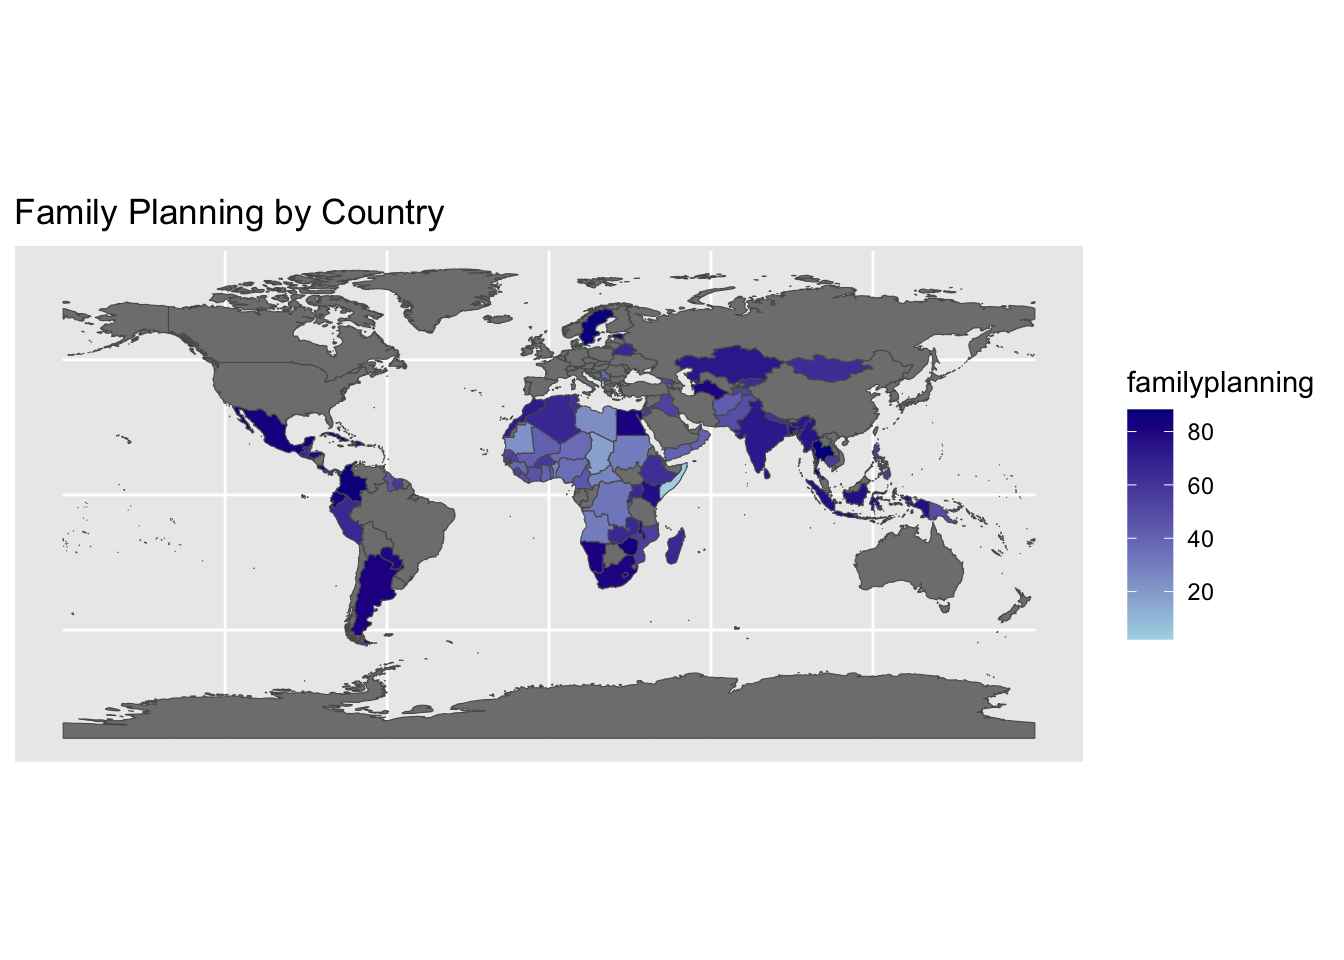
\includegraphics{Density map family planning.png}

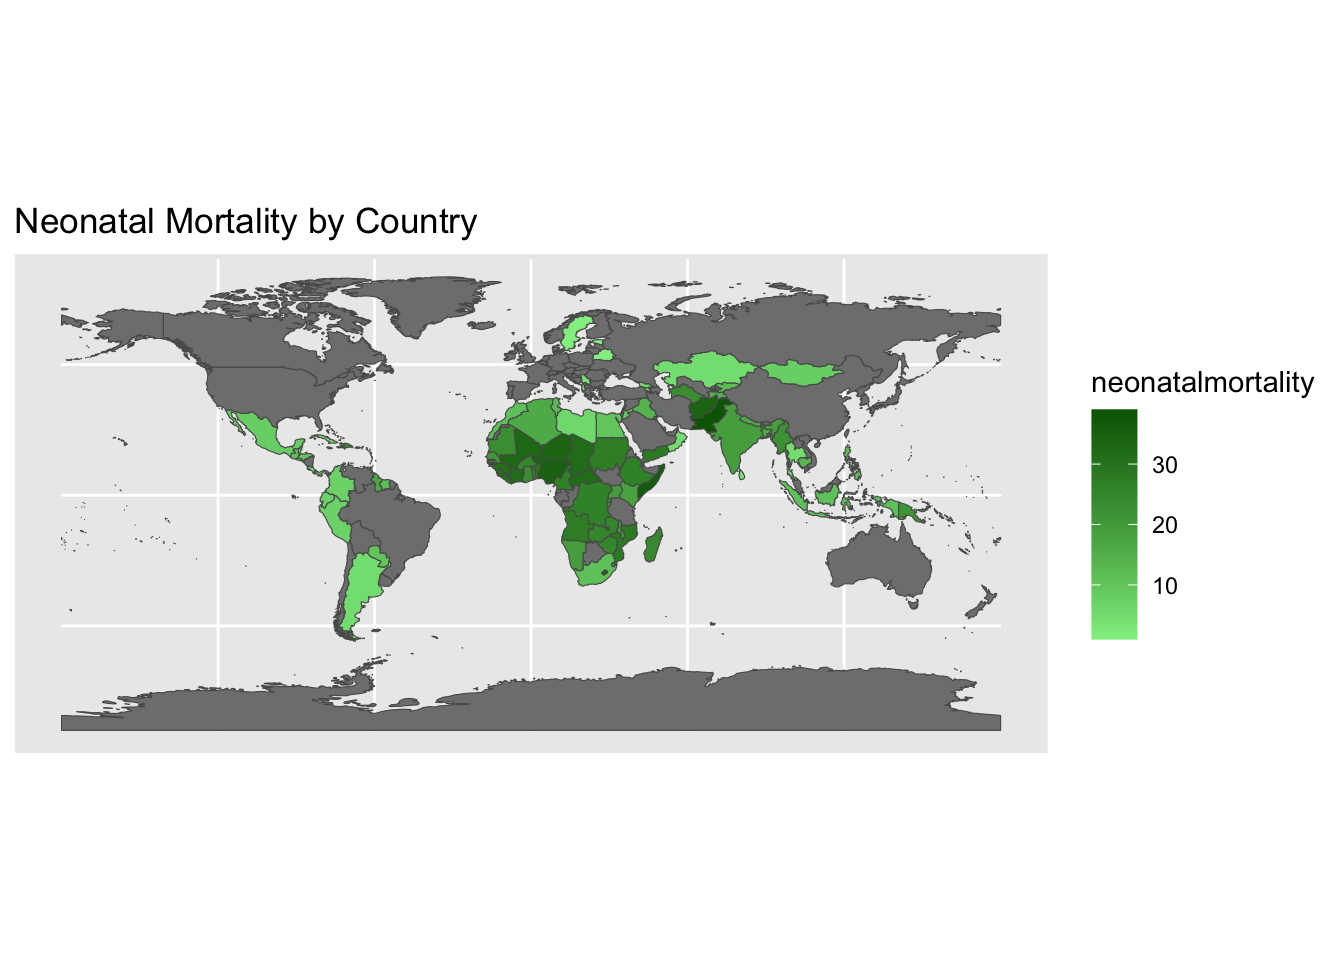
\includegraphics{density map neonatal.png}

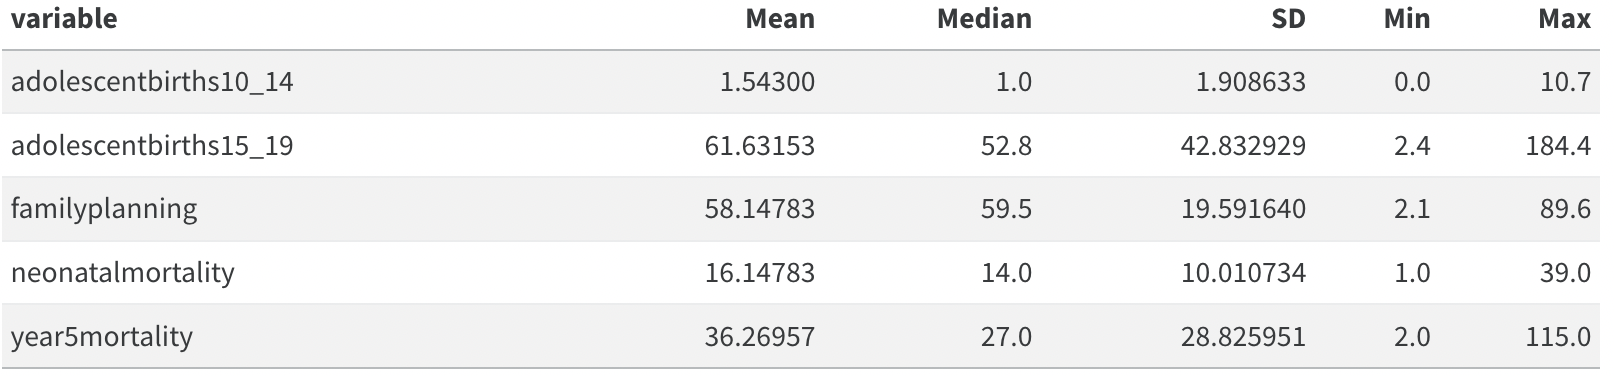
\includegraphics{Screen Shot 2023-12-07 at 6.45.03 PM.png}

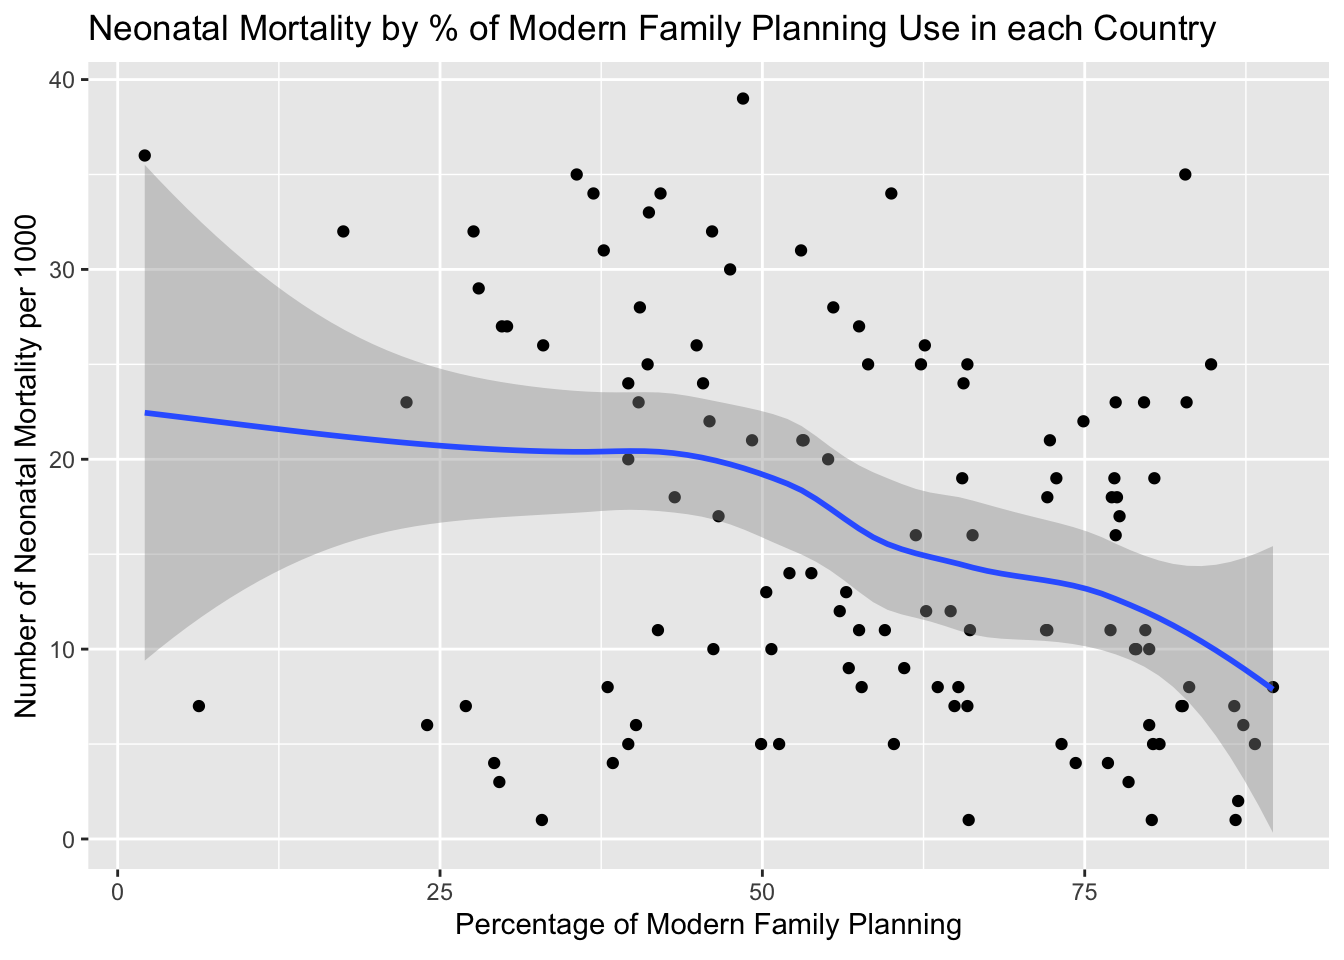
\includegraphics{neonatal.png}

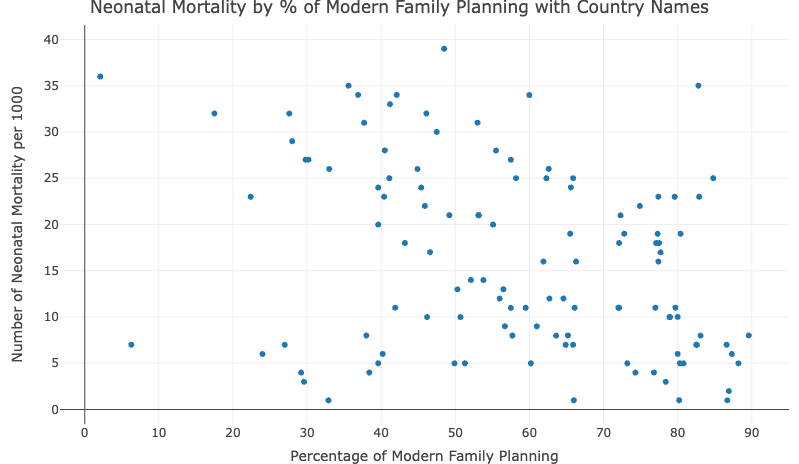
\includegraphics{newplot (2).png}

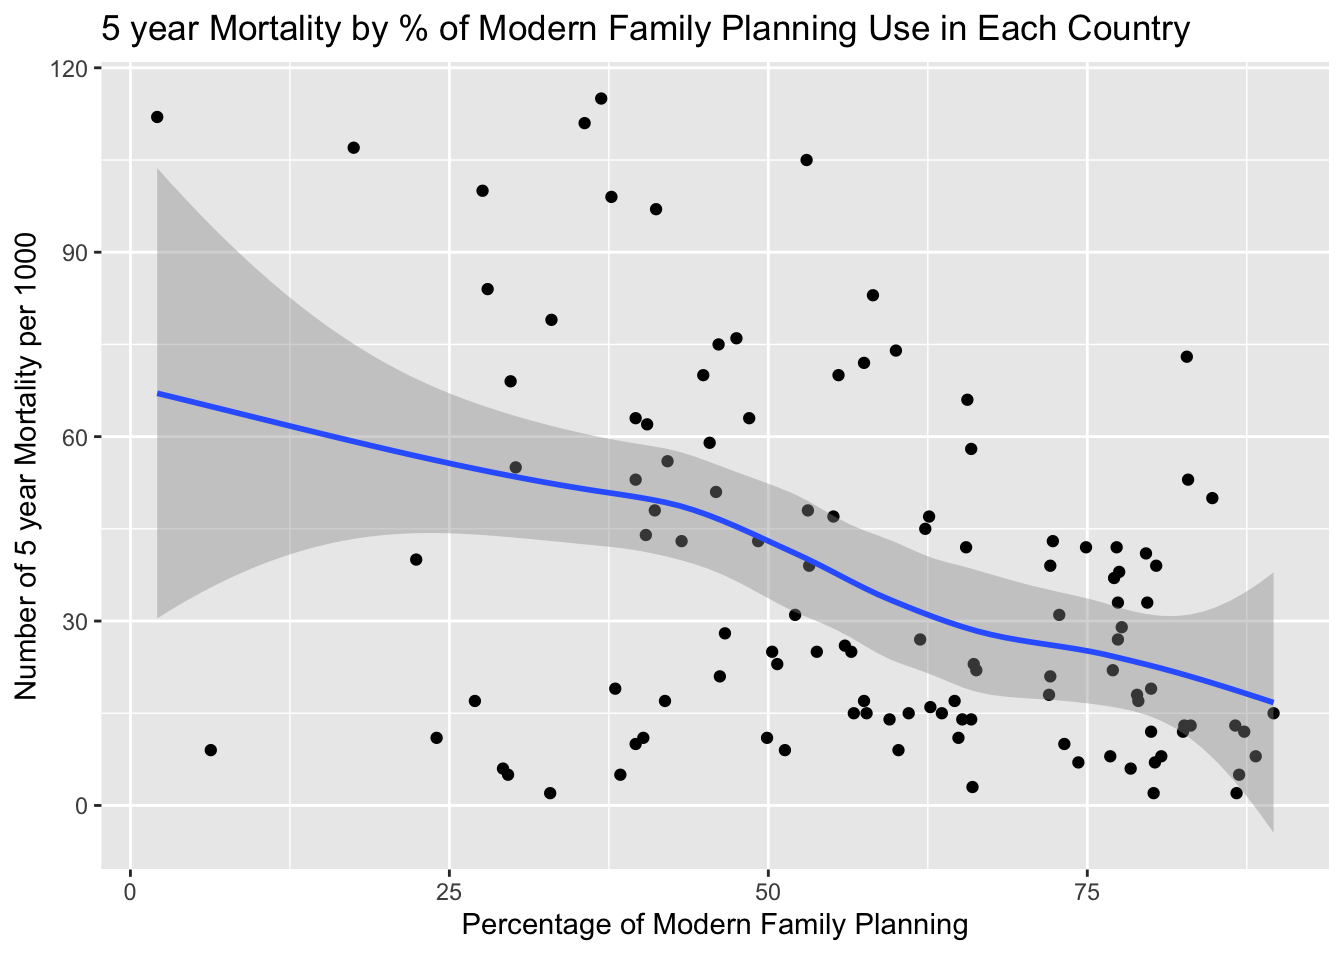
\includegraphics{5yeaer.png}

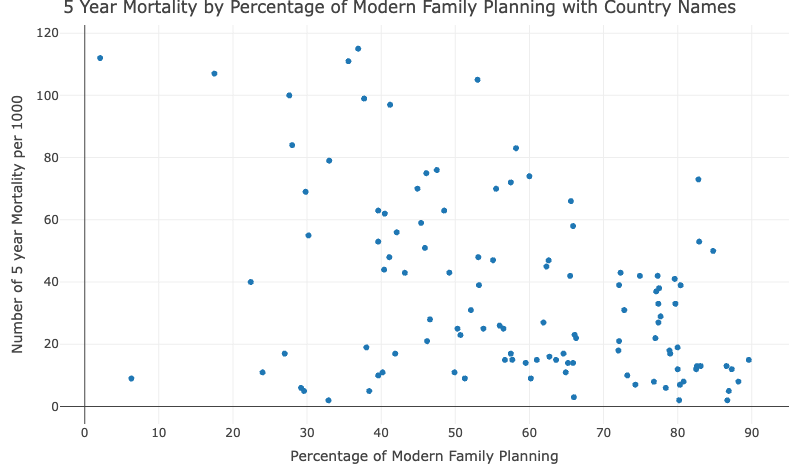
\includegraphics{newplot (3).png}

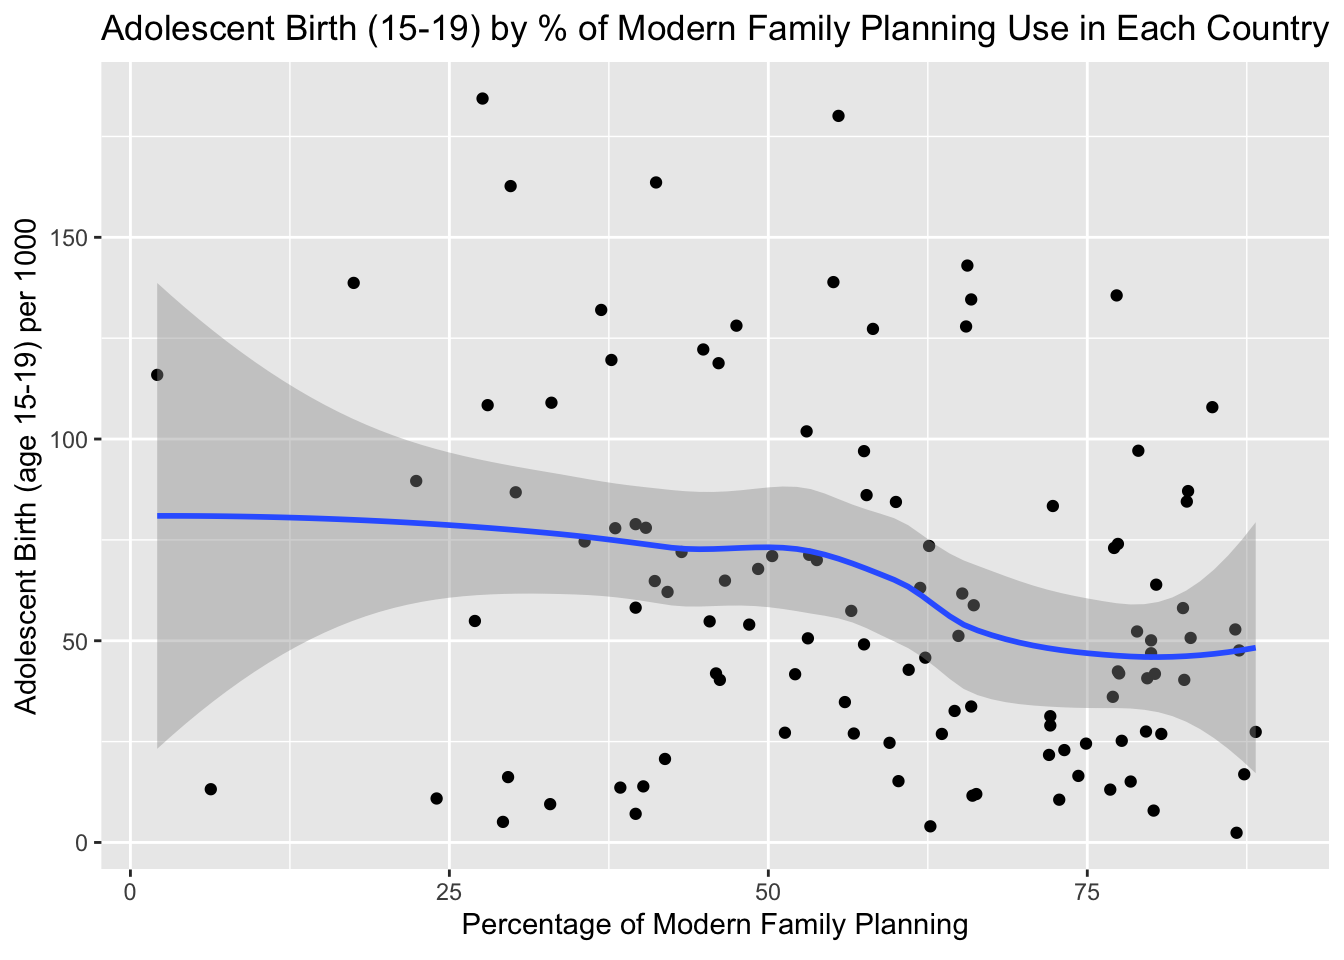
\includegraphics{adolescent 1519.png}

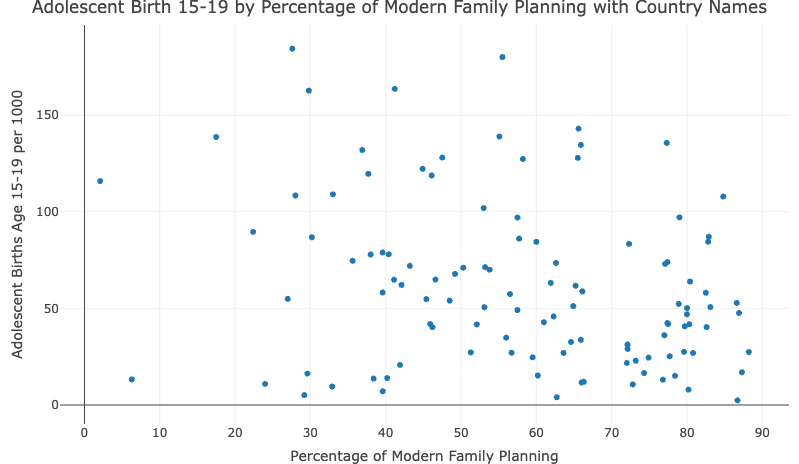
\includegraphics{newplot (4).png}

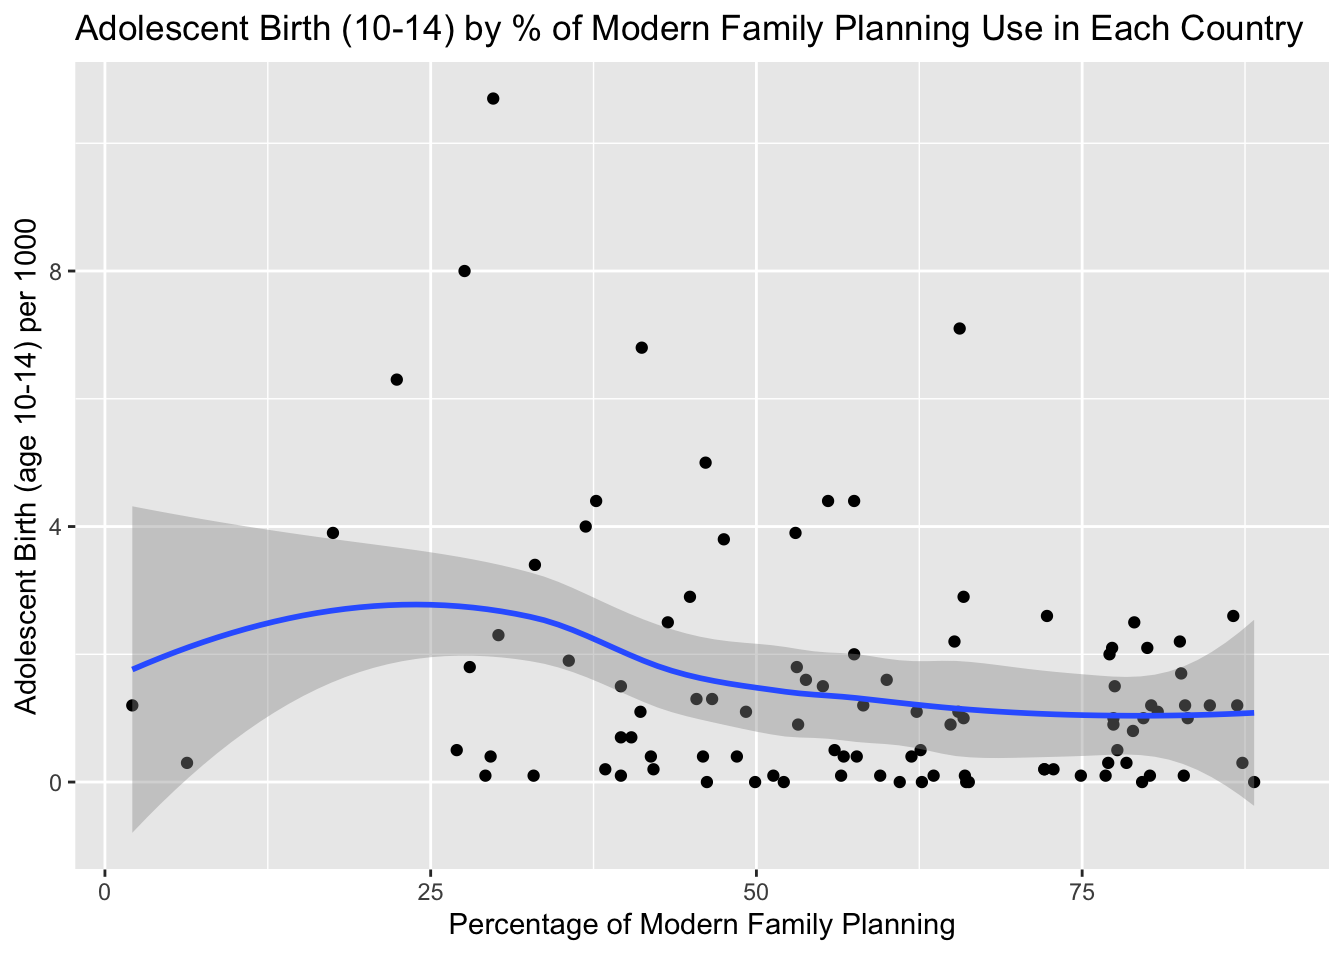
\includegraphics{adolescent 1014.png}

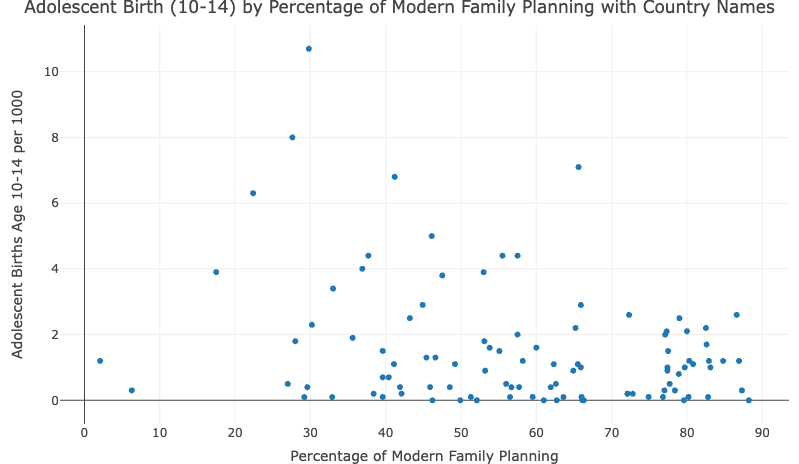
\includegraphics{newplot (1).png}

\hypertarget{conclusion}{%
\subsection{\texorpdfstring{\textbf{Conclusion}}{Conclusion}}\label{conclusion}}

There seems to be an association between increased family planning and
decreased neonatal mortality. This may be the case because more people
are able to choose when they want to have a baby and can be better
prepared for taking care of that baby when it is born when there is more
family planning. Another possible reason this could be true is because
when there is increased family planning, women are more capable of
planning when they want to have a baby and they can choose a time when
they are better able to get prenatal care to ensure the health of the
baby. There also seems to be an association between increased family
planning and 5 year mortality. Most likely the same reasons apply to why
this trend exists. One thing that was interesting was there did not seem
to be a strong association between adolescent birth rate of girls age
both 15-19 and 10-14 and family planning. This may be the case because
family planning methods are probably not marketed to adolescents at the
same level they are to adults. This can cause those who become sexually
active earlier in life to potentially be more likely to not use family
planning methods. It would be interesting to see the use of family
planning methods based on age and see if most adolescents regardless of
country do not use family planning methods which would explain the lack
of association. One potential limitation of this study is that there
might have been several countries that we eliminated that had no
neonatal mortality data and family planning data. These countries could
have strengthened our association because the countries which do not
have the capabilities of gathering this data may more likely be from a
lower income country and their access to family planning and health care
is limited. Therefore, it might be likely that they had low rates of
family planning and higher rates of neonatal mortality.



\end{document}
